%!TEX root = ../thesis_a4.tex
\chapter{State of the Art in Sampling-Based Composition}
\label{chap:sota}

As we move away from the symbolic leanings of the previous chapter and head towards audio content-based approaches to music generation, we pause once again from the deeper technical discourse to establish some context, both artistic and historic, before before providing a thorough definition of a concatenative synthesis - a form of synthesis that is rooted deeply in audio sampling - and its key works from the literature and community.

I use the term ``audio content-based'' here interchangeably here with sampling for good reason. The term actually stems from \acrshort{mir} parlance, used to dermarcate research that deals  directly with audio data and signals from those that analyse notated information and metadata \citep{Veltkamp2008, Casey2008a}. It also enforces the idea that we are working with elements extracted from found and realised objects and artefacts, which we will soon discover has a long and illustrious history as a creative aesthetic.  

\section{Artistic Context}

Historically, reusing existing material for the purposes of creating new works has been a widely practised technique in all branches of creative arts. The manifestations of these expressions can be wholly original and compelling or otherwise derivative, uninspiring and potentially copyright infringing depending on myriad factors, including the domain of the work, the scale of the reuse, and its cultural context.

In the visual arts, reusing or adapting existing material is most immediately understood in the use of collage, where existing works or parts thereof are assembled to create new artworks. Cubist artists such as George Braque and Pablo Picasso extensively referenced, appropriated and reinterpreted their own works and the works of others (\figref{fig:picasso}), as well as common found objects from their surroundings \citep{Greenberg1971}. Collage would later serve as direct inspiration for bricolage, reflecting wider postmodernist trends towards deconstructionism, self-referentiality,  and revisionism that include the practice of parody and pastiche \citep{Lochhead2002}. 

\begin{figure}
	\begin{center}
		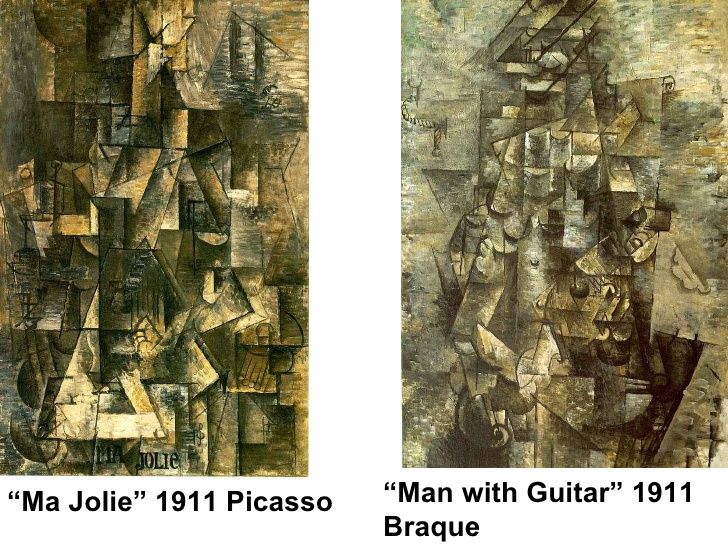
\includegraphics[width=0.9\textwidth]{ch04_sota/figures/picasso.png}
	\end{center}
	\caption[Cross-referential Cubist Works by Picasso and Braque]{Cross-referential Cubist Works by Picasso and Braque.}
	\label{fig:picasso}
\end{figure}
\subsection{Musique Concrète and Elektronische Musik}

In music and the sonic arts, its natural corollary came in the form of musique concrète \citep{Holmes2008}, a movement of composition stemming from the experiments of Pierre Schaeffer and, later, Pierre Henry at the studios of Radiodiffusion-Télévision Française in Paris during 1940s and 1950s \citep{Battier2007a}. In contrast to the artificially and electronically generated \textit{elektronische musik} spearheaded by Karlheinz Stockhausen at the \acrshort{wdr} in Cologne \citep{Collins2011a, Bates2009}, the French composers sought to conceive their works from existing recorded sound, including environmental sources like trains and speech. Seemingly unrelated and non-musical sounds were organised in such a way that the listener discovered the latent musical qualities and structure they inherently carry.

It is important to note that, in music composition, general appropriation of work predates these electronic advancements of technology. In Western art music, for example, composers like Bela Bartók – himself a musicologist - have often turned to folk music for its melodies and dance music styles \citep{Bartok1993}, while others such as Debussy \citep{Tamagawa1988} became enchanted by music from other cultures such as Javanese Gamelan, studying its form and incorporating the ideas into new pieces. Quotations, or direct lifting of melodies from other composers’ works, frequently crossing into classical, are also quite common, and has become a frequent, and often with the intention of being amusing, rudiment in jazz music practice \citep{Mangani2006}\footnote{\cite{Appel2002} recounts an anecdote of Stravinsky attending a Charlie Parker gig at his residency in the Birdland club in New York and ``[roaring] with delight, pounding his glass on the table'' on hearing a snippet of the opening of his Firebird Suite from the saxophone of the bebop pioneer.}.  For more on appropriation and quotation music a good reference is compiled by \cite{Metzer2003}.

\subsection{Granular Synthesis of Microsound}

Granular synthesis is composition at the microscale of sound - or to use Curtis Roads' term \textit{microsound} \citep{Roads2004}. It is a molecular viewpoint of music that \cite{Thomson2004} maintains finally promises the composer the possibility for ``total composition'', thereby dictating the parameters of everything from higher-order forms and structures all the way down to infinitesimal sonic minutiae.

It is generally agreed that the physicist Dennis Gabor first proposed the first quantum theory of sound that suggested ``large, complex sound events are composed of simple acoustic particles, or sonic grains' \citep{Miranda1995}. This was later reiterated and expanded on by Xenakis in \textit{Formalized Music} \citep{Bradshaw1973}, who laboriously arranged small snippets of tape material to produce \textit{Analogique B} (for 9 string instruments and tape, 1959) \citep{Robindore2009}.

Curtis Roads lays claim to developing the first digital implementation of granular synthesis \citep{Roads1998}, during the latter half of the 1970s (on punchcards!) and has composed with it and written about it capaciously ever since \citep{Roads1985, Roads1991, Roads1996, Roads2004} Barry Truax successfully achieved real-time granular synthesis during the 1980s with the composition of \textit{Riverrun} \citep{Truax1998}, using Poisson distributions and tendency masks to control the limits of typical granular parameters like frequency range, grain duration, modulation index, and delay.

Practically speaking, granular synthesis is, as \cite{Roads1998} suggests, a type of additive synthesis. Rather than mixing pure signals generated by oscillators to generate complex sounds, small `grains' (within the realm of 20-200ms) of existing sounds\footnote{Though these grains can, and often do, come from signal generators.} are superimposed to create dense amalgamations or `clouds' of sound grains \citep{Collins2011a, Thomson2004}. Nowadays granular synthesis is widespread in computer music practice and most music programming environments like Pd, Max and Reaktor, and even commercial synthesisers and \acrshort{daw}s,  provide extensive tools and tutorials for its pursuit. Listening to the works of glitch artists like Kim Cascone\footnote{The ideals of which are put forth in his influential manifesto ``The aesthetics of failure: ``Post-digital'' tendencies in contemporary computer music'', the most cited article in The Computer Music Journal \citep{Cascone2000}}\citep{Latartara2010}, or the more meditative washes of sound from drone and noise luminaries Tim Hecker or Fennesz, reveals an instantly recognisable application of the technique. 

I have used granular synthesis (\figref{fig:wolfcastle}) frequently in my own music for generating large indeterminate textural material from smaller fragments of composed musical ideas or interesting samples I have stumbled on. Recently this included a work  for violin, distortion and granular synthesis presented as part of the concert programme\footnote{Incidentally, Barry Truax premiered a new work during the same conference} of the \acrfull{smc} conference\footnote{\url{http://www.maynoothuniversity.ie/smc15/concert2.html}} as well as a quadrophonic soundscape that was installed at the Sonic Environments/\acrfull{acmc} satellite event that took place as part of \acrfull{nime} in 2016\footnote{\url{http://www.sonicenvironments.org/program.html}}. 

\begin{figure}
	\begin{center}
		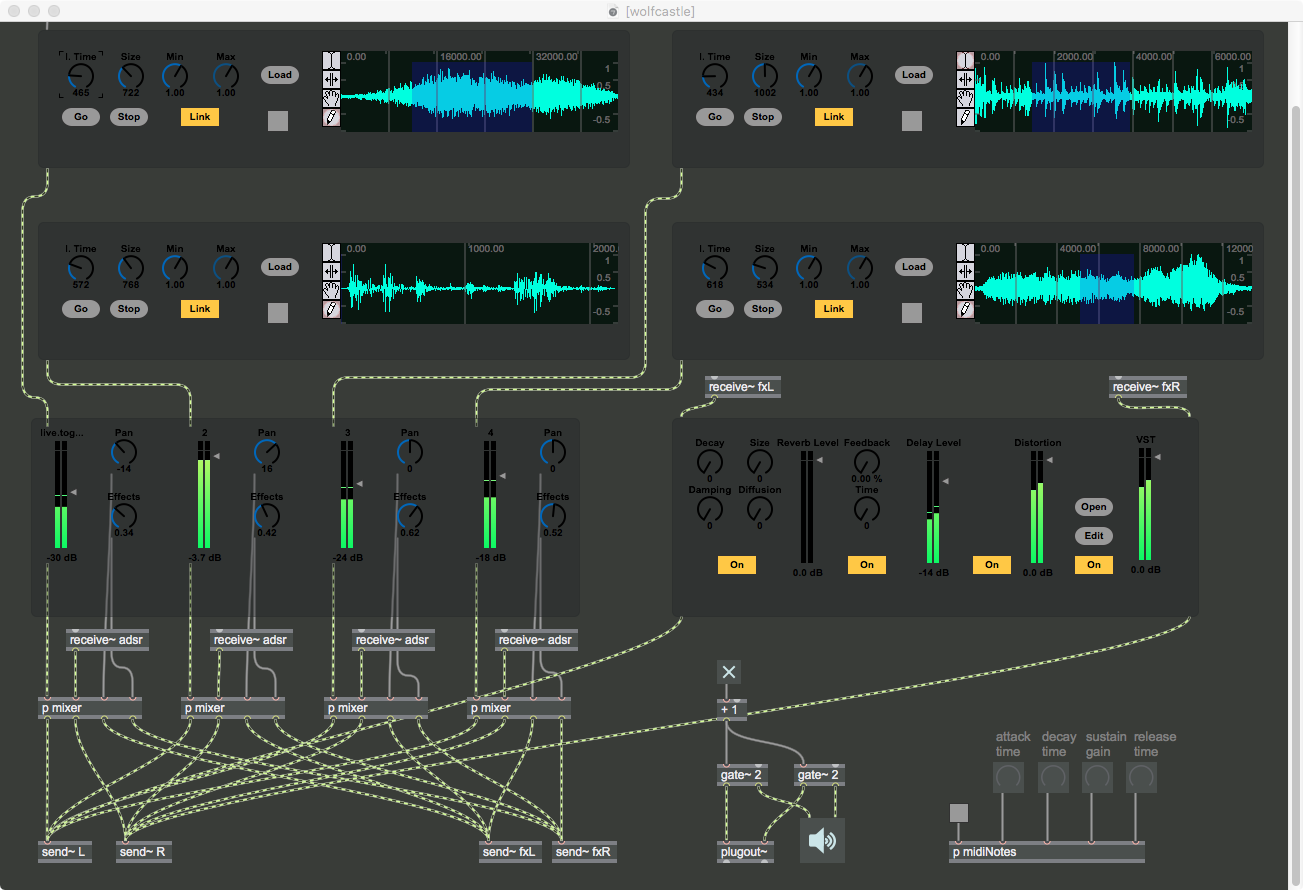
\includegraphics[width=1.0\textwidth]{ch04_sota/figures/wolfecastle.png}
	\end{center}
	\caption[Screenshot of my four-channel granular synthesiser for Max]{Screenshot of my four-channel granular synthesiser for Max\footnote{\url{https://github.com/carthach/Wolfcastle}}}
	\label{fig:wolfcastle}
\end{figure}

\subsection{Bring the Noise - Hip Hop Culture and the Birth of the Breakbeat}

In \chapref{chap:dancemusic} we briefly highlighted the contribution of DJ Kool Herc, who used two turntables to produce an extended looping, collage of drum sections (the breakbeats) from identical vinyl records \citep{Forman2004}. Kool Herc's contemporaries, Afrika Bambaataa and Grandmaster Flash observed his discovery and augmented it with more rudiments such as backspin, punch phrasing and, of course, record scratching which would widen the idiomatic vocabulary of \textit{turntablism} within the burgeoning subculture of hip-hop \citep{Smith2000}.

Vinyl would not reign king for too long however. The modern notion of sampling, at least in non-electroacoustic or contemporary composition circles, stems from the advent of the digital sampler and its eventual explosion of adaptation in hip-hop. The arrival of easy to use, self-contained hardware systems like the Akai \acrfull{mpc} offered the rhythmic sequencing facilities of the Roland TR range but with the groundbreaking ability to import one's own sounds (or more crucially, other artists' sounds), and all this with a reasonable price tag attached \citep{Rodgers2003}.

Hip-hop producers quickly latched onto the possibilities of these new tools. Artists such as Public Enemy and Beastie Boys, on albums like \textit{It Takes a Nation of Millions to Hold Us Back} and \textit{Paul's Boutique} respectively, painstakingly assembled bewildering permutations of musical samples, soundbites and miscellaneous other recorded materials that sought to supplant the many cultural references that permeated their lyrics \citep{Sewell2013, Sewell2014}. 

As was also identified in \chapref{chap:dancemusic}, the influence of hip-hop production would later inform the sample-heavy arrangements of jungle and drum and bass, in particular with its exhaustive re-rendering of the infamous ``Amen Break'' and James Brown's ``Funky Drummer''. In fact these breaks had already been dissected previously in hip-hop, long before UK producers got their digital surgical scalpels to them. The Amen Break appears on NWA's landmark gangster rap album \textit{Straight Outta Compton} and James Brown's ``Funky Drummer'' shows up on tracks by Run DMC and LL Cool J \citep{Frane2017}, leading \cite{Oliver2015} to observe that ``it is [Funky Drummer] sampled and recontextualized so extensively as to achieve near ubiquity in a wide range of popular music genres''.

Jungle and drum `n' bass was dealt with sufficiently in \chapref{chap:dancemusic} so it is hopefully not necessary to restate its relevance and impact on sample-based composition here. It is prudent to point out though that, since we are edging towards computational models and processes that automate audio content-based composition, that there is already a strong body of work that specifically addresses computational aspects of breakbeat analysis and its sequent generative synthesis. Nick Collins for example, has dedicated much of his academic dissemination to algorithms that can replicate the distinctive stuttering and glitching tropes that pervade in jungle, drum \& bass and post jungle emergent styles like breakcore \citep{Collins2001, Collins2002, Collins2006a}. Hockman has also devoted significant output to \acrshort{mir}-oriented analysis of timbral and rhythmic aspects unique to these styles \citep{Hockman2007, Hockman2012, Hockman2015}.

\pagebreak

\subsection{Plunderphonics and Metamusic}

\blockquote{``\textit{I quote from others the better to express myself}''}

\begin{flushright}
(Michel de Montaigne)
\end{flushright}

I think it's rather appropriate that the quote above I did not discover myself, instead I lifted it from an article dealing with the appropriation and quotation of other works in music \citep{Holm-Hudson1997}. The article is mostly concerned with the implications arising from the work of John Oswald, an artist who has gained much notoriety in his career by directly challenging musical copyright law for artistic gain. As hip-hop producers were trailblazing a new sound through intimate operation of the digital sampler, the inevitable direction was the bootlegging of other artists' music for creative repurposing, thus sparking the huge copyright debate. Record companies and legal representatives struggled to react to the huge paradigm shift in cultural production whose commercialisation was no longer under their total jurisdiction. The ethics of all this are outside the scope of this thesis obviously, but at least a few legal commentators at the time recognised that perhaps the long established laws governing creative ownership were no longer fit for purpose:

\blockcquote[]{Arewa1979}{``\textit{...copyright doctrine incorporates notions of Romantic authorship that assume independent and autonomous authorship and even genius in the creation of original musical works. This individualistic and autonomous vision of musical authorship, which is central to copyright law, has deemphasized the importance and continuity of musical borrowing practices generally}''}

Returning to John Oswald, who, capitalising on the polemics and its scope for creative interpretation, coined the name ``plunderphonics'' and set out his artistic intentions in a suitably subtitled 1985\footnote{Interesting then, that around this time Truax and Roads were still getting to grips with granular synthesis.} essay "Plunderphonics, or Audio Piracy as a Compositional Prerogative” \citep{Oswald1985}. The Canadian composer and media artist, inspired by the Dadaist cut-up literary technique practised by beat writer William S. Burroughs as well as sound collages by James Tenney \citep{Cox2004}, began to use tape-splicing techniques to create deliberately recognisable montages of other musical recordings, particularly pop music such as Michael Jackson or Led Zeppelin. If granular synthesis represents, as \cite{Thomson2004} indeed suggests,  a path to ``total composition'', then Oswald's modus operandi for composition is, as \cite{Holm-Hudson1997} describes it, the ``total importation'' of pieces involving ``reinterpretation or rehearing of existing recordings'' \citep{Cutler1994}.

Nowadays artists such as Girltalk and DJ Danger Mouse\footnote{Danger Mouse availed of the tendency in rap music to realise acapella versions of records for the purposes of remixing to create \textit{The Grey Album}: a well-received mashup of The Beatles' \textit{White Album} with Jay Z's \textit{The Black Album} \citep{Gunderson204}}\footnote{And much prior to that, experimental ensemble Negativland faced the legal backlash of record labels when they released the EP \textit{U2}, which contained misleading artwork and unauthorised sampling of the rock group, but ironically catapulted them into public notoriety \citep{herman1998politics, lysloff2003music}.} create extremely complex and multi-referential intersections of popular music harnessing the powerful beat matching and synchronisation capabilities of the modern \acrshort{daw} \citep{Humphrey2013}. The style has become known widely as ``mashups'' or ``bastard pop'' \citep{McGranahan2010} and straddles the fine line of what constitutes and can be protected under the auspices of fair usage \citep{Mongillo2009}, the very same doctrine that allows us to include images from other sources in this thesis in good faith.

Many computational works have emerged that explicitly mention and address the musical goals of mashup \citep{Tokui2008, Davies2013, Davies2014a, Davies2014b, Lee2015, Smith2015, Meroo-Peuela2017}, and we shall see that the direct consequence of concatenative synthesis can facilitate the realisation of elements of mashup.

\section{Concatenative Synthesis}

Recent associated research efforts in computer music, signal processing and music information retrieval afford us the opportunity to develop automated and intelligent systems that apply the aforementioned aesthetic of sampling and artistic reuse. 

The term ``concatenative synthesis'' (or musical mosaicing \citep{Zils2001}) has been extensively used to describe musical systems that create sound by recycling existing ones automatically, according to some well-defined set of criteria and algorithmic procedures \citep{Schwarz2000}. Concatenative synthesis can be considered the natural heir or big brother to granular synthesis. With concatenative synthesis, the grains of sound become “units” and are more related to musical scales of length, such as notes and phrases. Most importantly, descriptive information is attached to these units of sound: crucial features that allow the temporal, spectral, harmonic and timbral characteristics of the sound to determine the sequencing of final output. 

The criteria governing the procedure of concatenative synthesis is usually applied in relation to some reference sound or target that the composer wishes to emulate, and with this in mind, Bernardes gives a more thorough definition of the discipline:

\blockcquote[]{Bernardes2013}{``\textit{[Concatenative Synthesis] is a technique for synthesizing sounds by concatenating short audio segments (called units). It relies on a large database of segmented and descriptor-analyzed sound snippets (called corpus) to assemble a given target phrase by selecting the units that best match the target specification according to a distance measure in the descriptors}''}

In \chapref{chap:symbolic} we described symbolic methods that could take a seed or target rhythm pattern typical of dance music and replicate and variate it through similarity knowledge embedded in the fitness function of a \acrshort{ga}. With concatenative synthesis, we have a computational framework that can extend this notion of looping repetition and variation to audio. 

Just as granular synthesis invokes Heisenberg's Uncertainty Principle to blur the lines of time and frequency at the microscale of sound \citep{Truax2005}, we can view concatenative synthesis as a macroscale manipulation of the dichotomy between originality and theft determined by the scale of the unit - larger units of scale are more fully-formed but are more likely to be recognised as being lifted from other sources, while smaller units eventually approach granular levels of abstraction.
\section{Survey of Concatenative Synthesis Systems}

Other authors have previously provided insightful summaries of research trends in concatenative synthesis. In particular we suggest those by \cite{Schwarz2005, Schwarz2006b} and \cite{Sturm2006}. These surveys are over 10 years old however, so we offer here a more recent compendium of state of the art systems as we see them, based on our investigations of previous publications up until now.

\subsection{Unit Selection Synthesis of Speech}

Before music, concatenative synthesis has enjoyed successful application in the area of speech processing, specifically in the synthesis of \acrfull{tts}.

\cite{Hunt1996} were the first to propose unit selection synthesis using \acrfull{hmm}s as a means for combining phoneme units extracted from existing audio recordings of speech. \cite{Conkie1999} remarks that ``for unit selection synthesis, typically phone-based, it is possible to produce sentences that sound surprisingly natural and intelligible from a large database'. Since then many researchers \citep{Conkie1999, balestri1999choose, schroder2001emotional, Tihelka2010, Lakkavalli2010} and software systems \citep{black1994chatr, beutnagel1999t, Young2002} have cemented the popularity of the technique.

We will treat unit selection and \acrshort{hmm}s more thoroughly in \chapref{chap:pyconcat} but essentially \acrshort{hmm}s extend Markov chains (\secref{sec:markov_chains}) by assuming that the states in the state machine are now hidden but can output observable symbols. The Viterbi algorithm can return the most probable sequence of hidden states given a particular sequence of observed symbols. In concatenative synthesis, this maximum probabilistic model is inverted to facilitate minimal cost computations thereby encoding the dissimilarity of unit sounds.

Formulating the problem in terms of a \acrshort{hmm} enables us to capture two important contributors to a successful synthesis via the \textit{target cost} and the \textit{concatenation cost} (\figref{fig:target_concat_costs}). The target cost estimates the penalty of matching a corpus unit with the current target unit based on a target specification that stipulates factors like fundamental frequency or pitch, duration, position in the syllable and surrounding context of phonemes. The concatenation cost then estimates the quality of the join between two potential corpus units if they were to be selected, hence allowing a means of penalising selections that introduce unwanted jumps in energy and pitch (for example) that could lead to an unnatural sound. The Viterbi algorithm efficiently searches the state space of database units and outputs indices corresponding to the optimal state sequence for the target, based on a consolidated linear combination of the aforementioned costs \citep{Ob1995, Hunt1996}.

\begin{figure}
	\begin{center}
		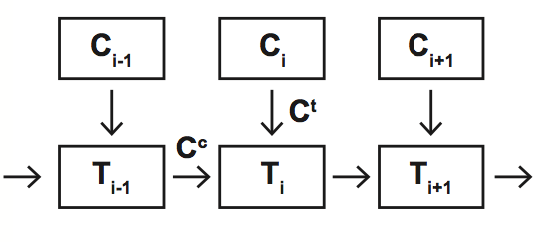
\includegraphics[width=0.6\textwidth]{ch04_sota/figures/costs.png}
	\end{center}
	\caption[Target  and concatenation costs in a text-to-speech Hidden Markov Model compared]{Target ($C^{t}$) and concatenation ($C^{c}$) costs in a \acrshort{tts} \acrshort{hmm} compared.}
	\label{fig:target_concat_costs}
\end{figure}

\subsection{Musical Concatenative Synthesis}
 
Schwarz directly applied Hunt’s HMM approach for musical purposes in his Caterpillar \citep{Schwarz2003}. He notes, however, that the HMM approach can be quite rigid for musical purposes since it produces one single optimised sequence without the ability to manipulate the individual units. To address these limitations, he reformulates the task into a constraint satisfaction problem which offers more flexibilities for interaction. A constraint satisfaction problem models a problem as a set of variables, values and a set of constraints that allows us to identify which combinations of variables and values are violations of those constraints, thus allowing us to quickly reduce large portions of the search space \citep{Russell2002}. 

Constraint satisfaction for concatenative synthesis was first introduced previously by \cite{Zils2001}, in what they describe as musical mosaicking or, to use their portmanteau, musaicing. They define two categories of constraints: segment constraints and sequence constraints. Segment constraints control aspects of individual units (much like the target cost in a \acrshort{hmm}-like system) based on their descriptor values. Sequence constraints apply globally, and affect aspects of time, continuity and overall distributions of units. The constraints can be applied manually by the user, or learned by modelling a target. The musically tailored “Adaptive Search” algorithm performs a heuristic search to minimise the total global cost generated by the constraint problem. One immediate advantage of this approach over the HMM is the ability to run the algorithm several times to generate alternative sequences, whereas the Viterbi process always outputs the most optimal solution.

 A simpler approach is presented in MatConcat \citep{Sturm2004}, using feature vectors comprising six descriptors and computing similarity metrics between target units and corpus units. Built for the Matlab scientific computing environment, the interface is quite involved, and the user has control over minute features such as descriptor tolerance ranges, relative descriptor weightings as well as window types and hop sizes of output transformations. On his website are short compositions generated by the author using excerpts from a Mahler symphony as a target, and resynthesised using various unrelated sound sets, for instance pop vocals, found sounds and solo instrumental recordings from saxophone and trumpet.

As concatenative synthesis methods matured, user modalities of interaction and control became more elaborate and real-time operations were introduced. One of the most compelling features of many concatenative systems is the concept of the interactive timbre space. With the release of CataRT \citep{Schwarz2006} the authors provided an interface (\figref{fig:catart}) that arranges the units in an interactive two-dimensional timbre space. The arrangement of these units is made according to a user-selectable descriptor on each axis. Instead of using a target sound file to inform the concatenation procedure, the user’s mouse cursor becomes the target. Sounds that are within a certain range of the mouse cursor are sequenced according to some triggering options (e.g. one-shot or  looped) and, most crucially, with real-time output.

\begin{figure}
\centering
\begin{subfigure}[b]{0.9\textwidth}
   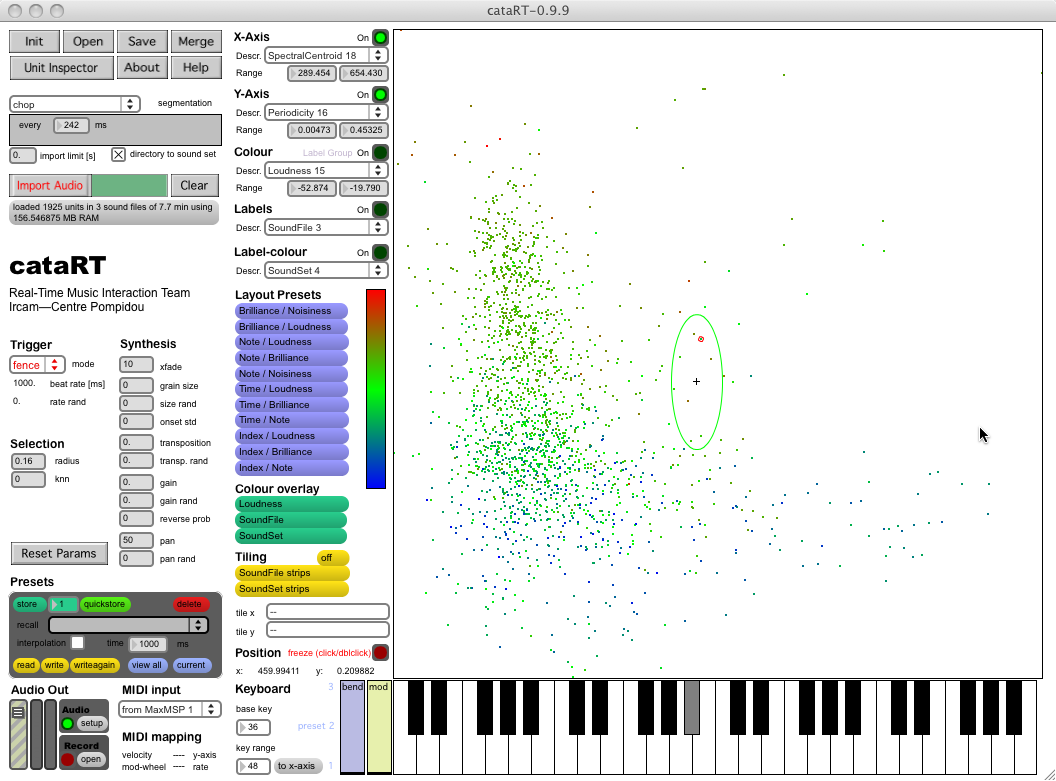
\includegraphics[width=1\linewidth]{ch04_sota/figures/catart.png}
   \caption{}
   \label{fig:catart} 
\end{subfigure}

\begin{subfigure}[b]{0.9\textwidth}
   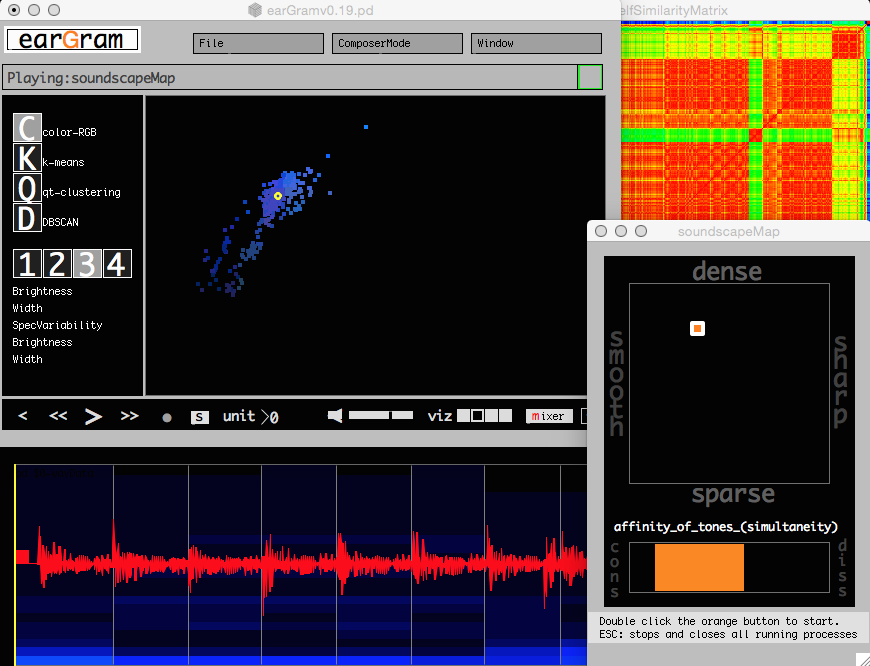
\includegraphics[width=1\linewidth]{ch04_sota/figures/eargram.png}
   \caption{}
   \label{fig:eargram}
\end{subfigure}

\caption[CataRT and Eargram]{(a) CataRT User Interface (Image from IRCAM), (b) earGram User Interface (Image from  SMC INESCTEC), both showing a clear realisation of an explorable 2D timbre space.}
\end{figure}

Bernardes takes inspiration from CataRT and also from Tristan Jehan’s Skeleton \citep{Jehan2005} to build his EarGram system for the Pure Data environment \citep{Bernardes2013}. Built on top of William Brent’s excellent feature extraction library timbreID \citep{Brent2010}, it adds a host of interesting features for visualisation and classification.  For instance, as well as the familiar waveform representation and previously described 2D timbre representation (\figref{fig:eargram}) (with various clustering modes and dimensionality reduction implementations), there are similarity matrices that show the temporal relations in the corpus over time. Some unique playback and sequencing modes also exist, such as the infiniteMode, which generates endless playback of sequences, and the soundscapeMap, which features an additional 2D control of parameters pertaining to sound scene design. Another system that adapts a 2D timbre space is Christian Frisson’s AudioGarden \citep{Frisson2010}, which offers two unique mapping procedures. The first of which, “Disc” mode, places units by assigning the length of the audio file to the radius of the unit from the centre, with the angle of rotation corresponding to a principal component of timbre (\acrshort{mfcc}s).  In the other Flower mode, a point of the sound is positioned in the space according to the average \acrshort{mfcc} coefficients of the entire sound file. Segments of the particular sound are arranged in chronological fashion around this centre point.

\begin{figure}
\centering
\begin{subfigure}[b]{0.9\textwidth}
   \includegraphics[width=1\linewidth]{ch04_sota/figures/audiogarden.png}
   \caption{}
   \label{fig:Ng1} 
\end{subfigure}

\begin{subfigure}[b]{0.9\textwidth}
   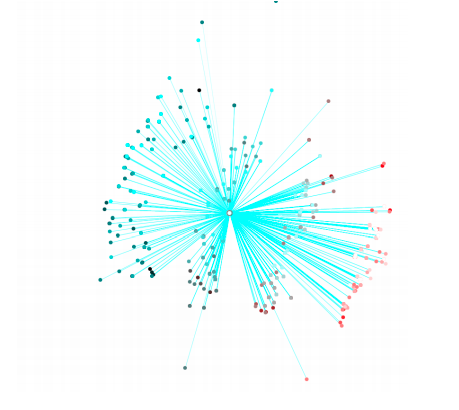
\includegraphics[width=1\linewidth]{ch04_sota/figures/audioguide.png}
   \caption{}
   \label{fig:audioguide}
\end{subfigure}

\caption[AudioGarden and AudioGuide Interfaces]{Two different visualisation of timbre: (a) AudioGarden ``Disc'' Visualisation (Image from \cite{Frisson2010}), (b) AudioGuide Clustering Visualisation around Target (Image from \cite{Schwarz2012}).}
\end{figure}

There have been some concatenative systems tailored specifically with rhythmic purposes in mind. Xiang proposes Granuloop \citep{Xiang2002} for automatically rearranging segments of 4 different drum loops into a 32 step sequence. Segmentation is done manually, without the aid of an automatic onset detector, using the Recycle sample editing software. Segmented sounds are compared using the inner product of the normalised frequency spectrum, supplemented with the weighted energy. These values become weights for a Markov-style probability transition matrix. Implemented in Pd, the user interacts by moving a joystick, in a 2D space, this then affects the overall probability weightings determining which loop segments are chosen. The system presents an interesting approach but is let down by its lack of online analysis. Ringomatic \citep{Aucouturier2005} is a real-time agent specifically tailored for combining drum tracks, expanding on many of the constraint-based ideas from their prior musaicing experiments. They applied the system to real-time performance following symbolic feature data extracted from a human \acrshort{midi} keyboard player. They cite, as an example, that a predominance of lower register notes in the keyboard performance applies an inverse constraint that creates complementary contrast by specifying that high-frequency heavy cymbal sounds should be concatenated.

As demonstrated in EarGram, concatenative synthesis has been considered useful in sound design tasks, allowing the sound designer to build rich and complex textures and environments that can be transformed in many ways both temporally and timbrally. Also in connection to sound design, \cite{Cardle2003} report on their Directed Sound Synthesis software as a means of providing sound designers and multimedia producers a method of automatically reusing and synthesising sound scenes in video. Users select one or more regions of an existing audio track, and can draw probability curves on the timeline to influence resynthesis of these regions (one curve per region) elsewhere. Soundscapes by \cite{Hoskinson2001}, in a nod to granular synthesis, refers to their segments as ”natural grains” and seek to synthesise endless streams of soundscapes. The selection scheme by which segments are chosen is based on a representation of each segment as a transition state in a Markov chain. Its interface features knobs and sliders for interactively controlling gain and parameters of multiple samples. To evaluate the platform they conducted an additional study \citep{Hoskinson2007} to reveal whether listening subjects found the concatenated sequences convincing compared to genuinely recorded soundscapes.

More specific and applied use cases of concatenative synthesis include \cite{Hackbarth2010}, who works intimately with the possibilities of concatenative synthesis in large scale music composition. He has worked with Schwarz to provide an alternative interface for exploring variations based on a force-directed graph (\figref{fig:audioguide}) to give a visual impression of the perceptual distances units in relation to a central target, not unlike the feedback we provided in our GenDrum instrument (see \chapref{chap:symbolic}). O’Connell describes a graphical system for Pd that demonstrates the use of higher level perceptual concepts like mood (happy vs sad) for informing selection in audio mosaics \citep{OConnell2011}.

Commercial implementations also exist for concatenative synthesis. Of particular note is Loopmash\footnote{\url{https://www.steinberg.net/en/products/mobile_apps/loopmash.html}}, a software plugin and mobile application for automatically creating mashups from existing looped content. The interface consists of a number of tracks in a timeline arrangement. One track is set as a master, and slices in the master are replaced with matching slices from the other slave tracks. Users interact by manipulating “similarity gain” sliders that control the influence of each track in the slice selection algorithm. Other applications exist more as \acrshort{midi} sampler systems attempting to model the performance qualities of natural sources such as orchestral ensembles\footnote{\url{https://www.synful.com/}} or the human voice\footnote{\url{https://www.vocaloid.com/en}}.

There are many other concatenative systems that are too numerous to discuss in detail here. \tabref{tab:concat_system_summary} compiles a summary of all the systems we came across in our research, with remarks on interaction and visualisation features, support for rhythm, and whether any user evaluation was carried out.

\newpage
\thispagestyle{empty}
\mbox{}



\begin{sidewaystable}
	\begin{threeparttable} 
		\ra{1.0}
%		\small
		\begin{centering}
			\begin{tabular}{l l l l l}
				\tabletop
				Author (Year) & Name & Evaluation & Interface & Rhythm or Tempo\\
				\tablemid			
				\cite{Schwarz2000}                & Caterpillar                   & No                     & 2D explorer                  & No             \\
				\cite{Zils2001}         & Musaicing                     & No                     & ?                            & Yes            \\
				Hazel(2001)               & Soundmosaic                   & No                     & Command Line                 & No             \\
				\cite{Hoskinson2001}      & Soundscapes                   & No                     & Waveform/Menus               & No             \\
				\cite{Xiang2002}          & Granuloop                     & No                     & 2D Controller                & Yes            \\
				\cite{Kobayashi}          & Sound Clustering Synthesis    & No                     & ?                            & No             \\
				\cite{Cardle2003}         & Directed Soundtrack Synthesis & Videos of use cases    & Waveform/Menus               & No             \\
				\cite{Lazier2003}         & MoSievius                     & No                     & ?                            & Looping        \\
				\cite{Sturm2004}          & MATConcat                     & No                     & Waveform/Menus               & No             \\
				\cite{Lindemann2007}		& Synful (Commercial)           & Not available          & Knobs/Sliders                & No             \\
				Casey (2005)                  & Soundspotter                  & Retrieval Accuracy     & Native Pure Data             & No             \\
				\cite{Aucouturier2005} & Ringomatic                    & User Experiment        & Lists/Menus                  & Drumming Tool  \\
				\cite{Simon2005}          & Audio Analogies               & Algorithm Performance  & None                         & No             \\
				\cite{Jehan2005}                  & Skeleton                      & Algorithmic evaluation & Waveform/Menus               &                \\
				\cite{Schwarz2006}                & CataRT                        & No                     & Timbre Space              & Looping option \\
			    Weiss et al. (2009)           & None                          & No                     & Waveform Segments            & No             \\
				\cite{Frisson2010}         & AudioGarden                   & No                     & Timbre Space / Waveform   & No             \\
				\cite{Hackbarth2010}			& AudioGuide                    & No                     & 2D CataRT based              & No             \\
				\cite{OConnell2011}             & None                          & Yes                    & Native Pure Data             & Looping demo   \\
				\cite{Bernardes2013}            & EarGram                       & Author's impressions   & Timbre Space and Matrices & Looping			\\	
				\tablebot		
			\end{tabular}
			\par \end{centering}		
		\begin{tablenotes}
			\small
%			\item[] ABBREVIATIONS: NA=Not applicable; GD=Group Delay, PDE=Probability Density Estimate
		\end{tablenotes}
			\caption[Summary of Existing Concatenative Sound Synthesis Systems]{Summary of Existing Concatenative Sound Synthesis Systems}
			\label{tab:concat_system_summary}
	\end{threeparttable}
\end{sidewaystable}

 